\documentclass[twoside]{book}

% Packages required by doxygen
\usepackage{fixltx2e}
\usepackage{calc}
\usepackage{doxygen}
\usepackage[export]{adjustbox} % also loads graphicx
\usepackage{graphicx}
\usepackage[utf8]{inputenc}
\usepackage{makeidx}
\usepackage{multicol}
\usepackage{multirow}
\PassOptionsToPackage{warn}{textcomp}
\usepackage{textcomp}
\usepackage[nointegrals]{wasysym}
\usepackage[table]{xcolor}

% Font selection
\usepackage[T1]{fontenc}
\usepackage[scaled=.90]{helvet}
\usepackage{courier}
\usepackage{amssymb}
\usepackage{sectsty}
\renewcommand{\familydefault}{\sfdefault}
\allsectionsfont{%
  \fontseries{bc}\selectfont%
  \color{darkgray}%
}
\renewcommand{\DoxyLabelFont}{%
  \fontseries{bc}\selectfont%
  \color{darkgray}%
}
\newcommand{\+}{\discretionary{\mbox{\scriptsize$\hookleftarrow$}}{}{}}

% Page & text layout
\usepackage{geometry}
\geometry{%
  a4paper,%
  top=2.5cm,%
  bottom=2.5cm,%
  left=2.5cm,%
  right=2.5cm%
}
\tolerance=750
\hfuzz=15pt
\hbadness=750
\setlength{\emergencystretch}{15pt}
\setlength{\parindent}{0cm}
\setlength{\parskip}{3ex plus 2ex minus 2ex}
\makeatletter
\renewcommand{\paragraph}{%
  \@startsection{paragraph}{4}{0ex}{-1.0ex}{1.0ex}{%
    \normalfont\normalsize\bfseries\SS@parafont%
  }%
}
\renewcommand{\subparagraph}{%
  \@startsection{subparagraph}{5}{0ex}{-1.0ex}{1.0ex}{%
    \normalfont\normalsize\bfseries\SS@subparafont%
  }%
}
\makeatother

% Headers & footers
\usepackage{fancyhdr}
\pagestyle{fancyplain}
\fancyhead[LE]{\fancyplain{}{\bfseries\thepage}}
\fancyhead[CE]{\fancyplain{}{}}
\fancyhead[RE]{\fancyplain{}{\bfseries\leftmark}}
\fancyhead[LO]{\fancyplain{}{\bfseries\rightmark}}
\fancyhead[CO]{\fancyplain{}{}}
\fancyhead[RO]{\fancyplain{}{\bfseries\thepage}}
\fancyfoot[LE]{\fancyplain{}{}}
\fancyfoot[CE]{\fancyplain{}{}}
\fancyfoot[RE]{\fancyplain{}{\bfseries\scriptsize Generated by Doxygen }}
\fancyfoot[LO]{\fancyplain{}{\bfseries\scriptsize Generated by Doxygen }}
\fancyfoot[CO]{\fancyplain{}{}}
\fancyfoot[RO]{\fancyplain{}{}}
\renewcommand{\footrulewidth}{0.4pt}
\renewcommand{\chaptermark}[1]{%
  \markboth{#1}{}%
}
\renewcommand{\sectionmark}[1]{%
  \markright{\thesection\ #1}%
}

% Indices & bibliography
\usepackage{natbib}
\usepackage[titles]{tocloft}
\setcounter{tocdepth}{3}
\setcounter{secnumdepth}{5}
\makeindex

% Hyperlinks (required, but should be loaded last)
\usepackage{ifpdf}
\ifpdf
  \usepackage[pdftex,pagebackref=true]{hyperref}
\else
  \usepackage[ps2pdf,pagebackref=true]{hyperref}
\fi
\hypersetup{%
  colorlinks=true,%
  linkcolor=blue,%
  citecolor=blue,%
  unicode%
}

% Custom commands
\newcommand{\clearemptydoublepage}{%
  \newpage{\pagestyle{empty}\cleardoublepage}%
}

\usepackage{caption}
\captionsetup{labelsep=space,justification=centering,font={bf},singlelinecheck=off,skip=4pt,position=top}

%===== C O N T E N T S =====

\begin{document}

% Titlepage & ToC
\hypersetup{pageanchor=false,
             bookmarksnumbered=true,
             pdfencoding=unicode
            }
\pagenumbering{alph}
\begin{titlepage}
\vspace*{7cm}
\begin{center}%
{\Large Wa\+SH Docs }\\
\vspace*{1cm}
{\large Generated by Doxygen 1.8.14}\\
\end{center}
\end{titlepage}
\clearemptydoublepage
\pagenumbering{roman}
\tableofcontents
\clearemptydoublepage
\pagenumbering{arabic}
\hypersetup{pageanchor=true}

%--- Begin generated contents ---
\chapter{Main Page}
\label{index}\hypertarget{index}{}\hypertarget{index_intro_sec}{}\section{Introduction}\label{index_intro_sec}
{\bfseries Wa}rwick {\bfseries S}mooth Particle {\bfseries H}ydrodynamics ({\bfseries Wa\+SH}) is a Domain Specific Language used for developing High Performance S\+PH simulations with built-\/in parallelisation using Open\+MP and C\+U\+DA.

This documentation has an \href{md_markdown_example_usecase.html}{\tt {\bfseries Introductory Simulation}} to show you how to use the Wa\+SH A\+PI to write a fully-\/functional S\+PH simulation.

Before that, you must make sure all the required libraries and dependencies are installed. Just follow the \href{md_markdown_installation.html}{\tt {\bfseries Installation Steps}} here.

\section*{$<$$<$$<$$<$$<$$<$$<$ H\+E\+AD }\hypertarget{index_step1}{}\subsection{Step 1\+:}\label{index_step1}
The link text \begin{quote}
\begin{quote}
\begin{quote}
\begin{quote}
\begin{quote}
\begin{quote}
\begin{quote}
d9b2d93 (new website)\end{quote}
\end{quote}
\end{quote}
\end{quote}
\end{quote}
\end{quote}
\end{quote}

\chapter{markdown\+\_\+test}
\label{md_markdown_markdown_test}
\Hypertarget{md_markdown_markdown_test}
Try to put a blank line before...

\section*{Heading}

...and after a heading. 
\chapter{cs407}
\label{md__dcs_20_u2002000_4thYearProject_wash_README}
\Hypertarget{md__dcs_20_u2002000_4thYearProject_wash_README}
Wa\+SH -\/ $\ast$$\ast$\+\_\+\+\_\+\+Wa\+\_\+\+\_\+$\ast$$\ast$ rwick $\ast$$\ast$\+\_\+\+\_\+\+S\+\_\+\+\_\+$\ast$$\ast$ mooth $\ast$$\ast$\+\_\+\+\_\+\+H\+\_\+\+\_\+$\ast$$\ast$ ydro

Wa\+SH is a Domain Specific Language on top of C++ for Smooth Particle Hydrodynamics simulations to help developers and researchers best utilise all their available hardware, using combinations of C\+U\+DA, Open\+MP, and M\+PI. 
\chapter{Hierarchical Index}
\section{Class Hierarchy}
This inheritance list is sorted roughly, but not completely, alphabetically\+:\begin{DoxyCompactList}
\item \contentsline{section}{wash\+:\+:Generic\+File\+Reader}{\pageref{classwash_1_1GenericFileReader}}{}
\begin{DoxyCompactList}
\item \contentsline{section}{wash\+:\+:A\+S\+C\+I\+I\+Reader}{\pageref{classwash_1_1ASCIIReader}}{}
\end{DoxyCompactList}
\item \contentsline{section}{wash\+:\+:Generic\+File\+Writer}{\pageref{classwash_1_1GenericFileWriter}}{}
\begin{DoxyCompactList}
\item \contentsline{section}{wash\+:\+:A\+S\+C\+I\+I\+Writer}{\pageref{classwash_1_1ASCIIWriter}}{}
\end{DoxyCompactList}
\item \contentsline{section}{wash\+:\+:Particle}{\pageref{classwash_1_1Particle}}{}
\item \contentsline{section}{wash\+:\+:Vec$<$ T, dim $>$}{\pageref{classwash_1_1Vec}}{}
\item \contentsline{section}{wash\+:\+:Vec$<$ double, D\+IM $>$}{\pageref{classwash_1_1Vec}}{}
\end{DoxyCompactList}

\chapter{Class Index}
\doxysection{Class List}
Here are the classes, structs, unions and interfaces with brief descriptions\+:\begin{DoxyCompactList}
\item\contentsline{section}{\mbox{\hyperlink{classwash_1_1Particle}{wash\+::\+Particle}} }{\pageref{classwash_1_1Particle}}{}
\item\contentsline{section}{\mbox{\hyperlink{classwash_1_1Vec}{wash\+::\+Vec$<$ T, dim $>$}} }{\pageref{classwash_1_1Vec}}{}
\end{DoxyCompactList}

\chapter{File Index}
\section{File List}
Here is a list of all documented files with brief descriptions\+:\begin{DoxyCompactList}
\item\contentsline{section}{/dcs/20/u2002000/4th\+Year\+Project/wash/src/examples/3d\+\_\+fluid\+\_\+sim/{\bfseries fluid\+\_\+sim.\+hpp} }{\pageref{3d__fluid__sim_2fluid__sim_8hpp}}{}
\item\contentsline{section}{/dcs/20/u2002000/4th\+Year\+Project/wash/src/examples/ca\+\_\+fluid\+\_\+sim/{\bfseries fluid\+\_\+sim.\+hpp} }{\pageref{ca__fluid__sim_2fluid__sim_8hpp}}{}
\item\contentsline{section}{/dcs/20/u2002000/4th\+Year\+Project/wash/src/examples/ca\+\_\+fluid\+\_\+sim/{\bfseries generated\+\_\+enums.\+hpp} }{\pageref{generated__enums_8hpp}}{}
\item\contentsline{section}{/dcs/20/u2002000/4th\+Year\+Project/wash/src/examples/ca\+\_\+fluid\+\_\+sim/{\bfseries kernels.\+hpp} }{\pageref{examples_2ca__fluid__sim_2kernels_8hpp}}{}
\item\contentsline{section}{/dcs/20/u2002000/4th\+Year\+Project/wash/src/examples/sedov\+\_\+blast\+\_\+wave/{\bfseries box.\+hpp} }{\pageref{box_8hpp}}{}
\item\contentsline{section}{/dcs/20/u2002000/4th\+Year\+Project/wash/src/examples/sedov\+\_\+blast\+\_\+wave/{\bfseries consts.\+hpp} }{\pageref{consts_8hpp}}{}
\item\contentsline{section}{/dcs/20/u2002000/4th\+Year\+Project/wash/src/examples/sedov\+\_\+blast\+\_\+wave/{\bfseries force.\+hpp} }{\pageref{force_8hpp}}{}
\item\contentsline{section}{/dcs/20/u2002000/4th\+Year\+Project/wash/src/examples/sedov\+\_\+blast\+\_\+wave/{\bfseries init.\+hpp} }{\pageref{init_8hpp}}{}
\item\contentsline{section}{/dcs/20/u2002000/4th\+Year\+Project/wash/src/examples/sedov\+\_\+blast\+\_\+wave/{\bfseries neighbors.\+hpp} }{\pageref{neighbors_8hpp}}{}
\item\contentsline{section}{/dcs/20/u2002000/4th\+Year\+Project/wash/src/examples/sedov\+\_\+blast\+\_\+wave/{\bfseries update.\+hpp} }{\pageref{update_8hpp}}{}
\item\contentsline{section}{/dcs/20/u2002000/4th\+Year\+Project/wash/src/examples/sedov\+\_\+solution/\mbox{\hyperlink{sedov__computer_8cpp}{sedov\+\_\+computer.\+cpp}} }{\pageref{sedov__computer_8cpp}}{}
\item\contentsline{section}{/dcs/20/u2002000/4th\+Year\+Project/wash/src/examples/sedov\+\_\+solution/\mbox{\hyperlink{sedov__computer_8hpp}{sedov\+\_\+computer.\+hpp}} \\*This class produces 1d solutions for a sedov blast wave propagating through a density gradient\+: rho = rho$\ast$$\ast$(-\/omega) , in planar(1\+D), cylindrical(2\+D) or spherical geometry(3\+D) for the \textquotesingle{}standard\textquotesingle{}, \textquotesingle{}singular\textquotesingle{} and \textquotesingle{}vaccum\textquotesingle{} cases }{\pageref{sedov__computer_8hpp}}{}
\item\contentsline{section}{/dcs/20/u2002000/4th\+Year\+Project/wash/src/gen/\mbox{\hyperlink{finder_8cpp}{finder.\+cpp}} \\*Implements the Find Wash Function funtionality }{\pageref{finder_8cpp}}{}
\item\contentsline{section}{/dcs/20/u2002000/4th\+Year\+Project/wash/src/gen/\mbox{\hyperlink{finder_8hpp}{finder.\+hpp}} \\*Find Wash Function is a small tool/plugin which scans through program source code and reports a) wash function declarations and b) wash function calls }{\pageref{finder_8hpp}}{}
\item\contentsline{section}{/dcs/20/u2002000/4th\+Year\+Project/wash/src/gen/\mbox{\hyperlink{finder__plugin_8cpp}{finder\+\_\+plugin.\+cpp}} \\*Implements the Find Wash Function as a plugin for clang compiler }{\pageref{finder__plugin_8cpp}}{}
\item\contentsline{section}{/dcs/20/u2002000/4th\+Year\+Project/wash/src/gen/\mbox{\hyperlink{finder__tool_8cpp}{finder\+\_\+tool.\+cpp}} \\*Runs the Find Wash Function as a standalone clang tool on passed in code }{\pageref{finder__tool_8cpp}}{}
\item\contentsline{section}{/dcs/20/u2002000/4th\+Year\+Project/wash/src/gen/\mbox{\hyperlink{inspect_8cpp}{inspect.\+cpp}} \\*Inspecting the contents of Wa\+SH C++ files }{\pageref{inspect_8cpp}}{}
\item\contentsline{section}{/dcs/20/u2002000/4th\+Year\+Project/wash/src/gen/{\bfseries inspect.\+hpp} }{\pageref{inspect_8hpp}}{}
\item\contentsline{section}{/dcs/20/u2002000/4th\+Year\+Project/wash/src/gen/\mbox{\hyperlink{kernels_8cpp}{kernels.\+cpp}} \\*Implementations for the kernel plugin/tool }{\pageref{kernels_8cpp}}{}
\item\contentsline{section}{/dcs/20/u2002000/4th\+Year\+Project/wash/src/gen/{\bfseries kernels.\+hpp} }{\pageref{gen_2kernels_8hpp}}{}
\item\contentsline{section}{/dcs/20/u2002000/4th\+Year\+Project/wash/src/io/{\bfseries ascii.\+hpp} }{\pageref{ascii_8hpp}}{}
\item\contentsline{section}{/dcs/20/u2002000/4th\+Year\+Project/wash/src/io/{\bfseries hdf5.\+hpp} }{\pageref{hdf5_8hpp}}{}
\item\contentsline{section}{/dcs/20/u2002000/4th\+Year\+Project/wash/src/io/{\bfseries io.\+hpp} }{\pageref{io_8hpp}}{}
\item\contentsline{section}{/dcs/20/u2002000/4th\+Year\+Project/wash/src/io/{\bfseries none.\+hpp} }{\pageref{none_8hpp}}{}
\item\contentsline{section}{/dcs/20/u2002000/4th\+Year\+Project/wash/src/io/\mbox{\hyperlink{read__ascii_8cpp}{read\+\_\+ascii.\+cpp}} \\*Reads in an ascii plaintext file into the simulation as a checkpoint }{\pageref{read__ascii_8cpp}}{}
\item\contentsline{section}{/dcs/20/u2002000/4th\+Year\+Project/wash/src/io/\mbox{\hyperlink{read__hdf5_8cpp}{read\+\_\+hdf5.\+cpp}} \\*Reads in a H\+D\+F5 file with the intention of constructing a simulation state from which to continue }{\pageref{read__hdf5_8cpp}}{}
\item\contentsline{section}{/dcs/20/u2002000/4th\+Year\+Project/wash/src/io/\mbox{\hyperlink{write__ascii_8cpp}{write\+\_\+ascii.\+cpp}} \\*Writes the simulation data to an ascii plaintext file in C\+SV format }{\pageref{write__ascii_8cpp}}{}
\item\contentsline{section}{/dcs/20/u2002000/4th\+Year\+Project/wash/src/io/\mbox{\hyperlink{write__hdf5_8cpp}{write\+\_\+hdf5.\+cpp}} \\*Write out the simulation state serially to a H\+D\+F5 file }{\pageref{write__hdf5_8cpp}}{}
\item\contentsline{section}{/dcs/20/u2002000/4th\+Year\+Project/wash/src/io/\mbox{\hyperlink{write__hdf5__dump_8cpp}{write\+\_\+hdf5\+\_\+dump.\+cpp}} \\*Writes out to a H\+D\+F5 file in a similar format to sedov. With a singular dump file contianing each iteration as a separate group, with attributes controlling time\+Step and iteration no }{\pageref{write__hdf5__dump_8cpp}}{}
\item\contentsline{section}{/dcs/20/u2002000/4th\+Year\+Project/wash/src/wash/{\bfseries enum.\+h} }{\pageref{enum_8h}}{}
\item\contentsline{section}{/dcs/20/u2002000/4th\+Year\+Project/wash/src/wash/{\bfseries particle.\+hpp} }{\pageref{wash_2particle_8hpp}}{}
\item\contentsline{section}{/dcs/20/u2002000/4th\+Year\+Project/wash/src/wash/{\bfseries util.\+hpp} }{\pageref{util_8hpp}}{}
\item\contentsline{section}{/dcs/20/u2002000/4th\+Year\+Project/wash/src/wash/{\bfseries vector.\+hpp} }{\pageref{vector_8hpp}}{}
\item\contentsline{section}{/dcs/20/u2002000/4th\+Year\+Project/wash/src/wash/{\bfseries wash.\+hpp} }{\pageref{wash_2wash_8hpp}}{}
\item\contentsline{section}{/dcs/20/u2002000/4th\+Year\+Project/wash/src/wisb/{\bfseries particle.\+hpp} }{\pageref{wisb_2particle_8hpp}}{}
\item\contentsline{section}{/dcs/20/u2002000/4th\+Year\+Project/wash/src/wisb/{\bfseries particle\+\_\+data.\+hpp} }{\pageref{particle__data_8hpp}}{}
\item\contentsline{section}{/dcs/20/u2002000/4th\+Year\+Project/wash/src/wisb/{\bfseries wash.\+hpp} }{\pageref{wisb_2wash_8hpp}}{}
\end{DoxyCompactList}

\chapter{Class Documentation}
\hypertarget{classwash_1_1ASCIIReader}{}\section{wash\+:\+:A\+S\+C\+I\+I\+Reader Class Reference}
\label{classwash_1_1ASCIIReader}\index{wash\+::\+A\+S\+C\+I\+I\+Reader@{wash\+::\+A\+S\+C\+I\+I\+Reader}}
Inheritance diagram for wash\+:\+:A\+S\+C\+I\+I\+Reader\+:\begin{figure}[H]
\begin{center}
\leavevmode
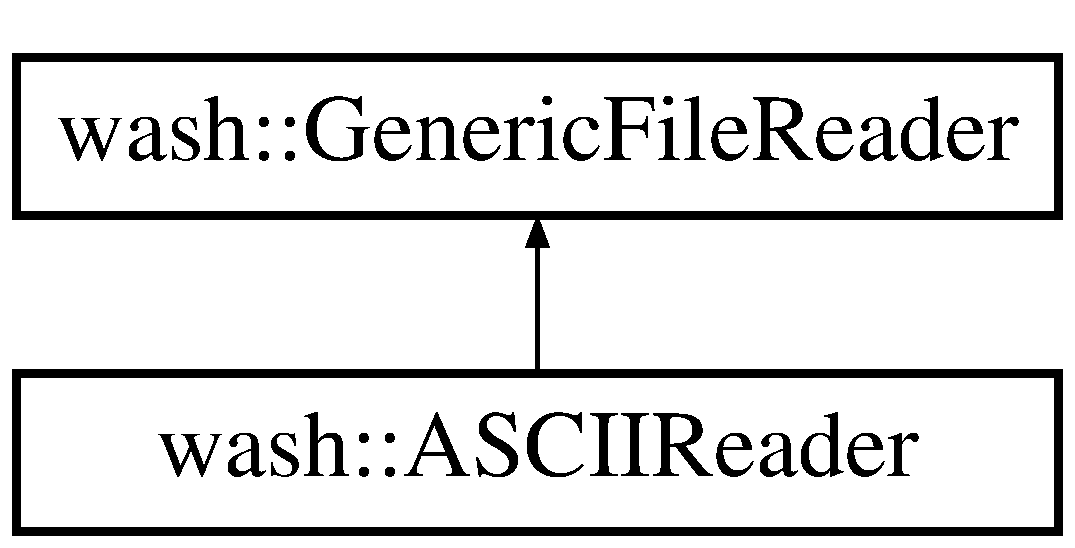
\includegraphics[height=2.000000cm]{classwash_1_1ASCIIReader}
\end{center}
\end{figure}
\subsection*{Public Member Functions}
\begin{DoxyCompactItemize}
\item 
\mbox{\Hypertarget{classwash_1_1ASCIIReader_ae9248e52a7bcf48e54b1cd63cebf3d42}\label{classwash_1_1ASCIIReader_ae9248e52a7bcf48e54b1cd63cebf3d42}} 
void {\bfseries read\+\_\+iteration} (const size\+\_\+t iteration\+\_\+number) const override
\end{DoxyCompactItemize}


The documentation for this class was generated from the following files\+:\begin{DoxyCompactItemize}
\item 
/dcs/20/u2002000/4th\+Year\+Project/wash/src/io/ascii.\+hpp\item 
/dcs/20/u2002000/4th\+Year\+Project/wash/src/io/\mbox{\hyperlink{read__ascii_8cpp}{read\+\_\+ascii.\+cpp}}\end{DoxyCompactItemize}

\hypertarget{classwash_1_1ASCIIWriter}{}\section{wash\+:\+:A\+S\+C\+I\+I\+Writer Class Reference}
\label{classwash_1_1ASCIIWriter}\index{wash\+::\+A\+S\+C\+I\+I\+Writer@{wash\+::\+A\+S\+C\+I\+I\+Writer}}
Inheritance diagram for wash\+:\+:A\+S\+C\+I\+I\+Writer\+:\begin{figure}[H]
\begin{center}
\leavevmode
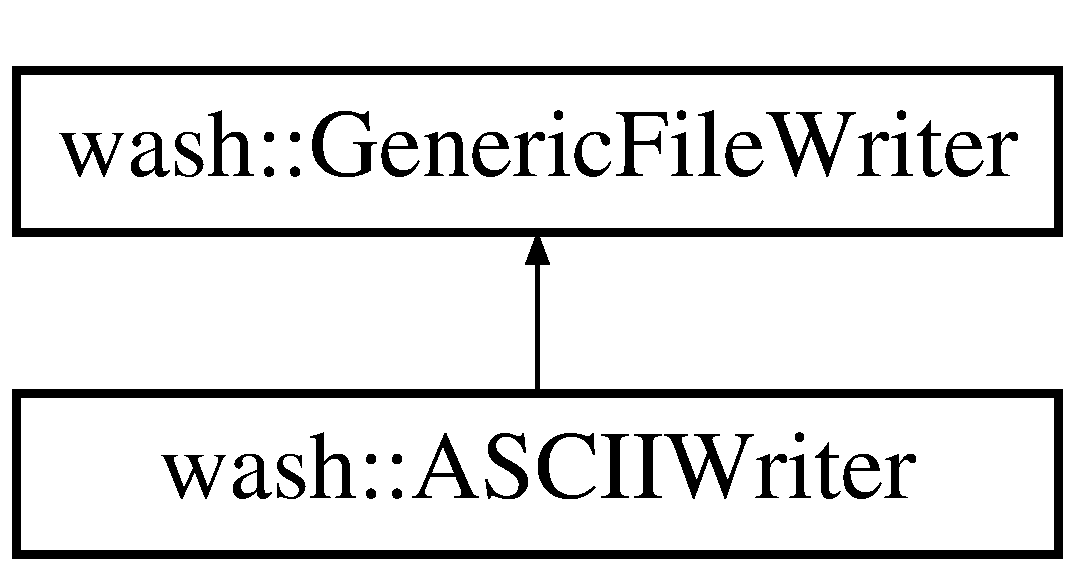
\includegraphics[height=2.000000cm]{classwash_1_1ASCIIWriter}
\end{center}
\end{figure}
\subsection*{Public Member Functions}
\begin{DoxyCompactItemize}
\item 
\mbox{\Hypertarget{classwash_1_1ASCIIWriter_ab6594fb85b025fe5ab21114be676a22b}\label{classwash_1_1ASCIIWriter_ab6594fb85b025fe5ab21114be676a22b}} 
void {\bfseries begin\+\_\+iteration} (const size\+\_\+t iterationc, const std\+::string path) override
\item 
\mbox{\Hypertarget{classwash_1_1ASCIIWriter_ae0d91c1d0a7af5dfb8d0e36b33b7d3c7}\label{classwash_1_1ASCIIWriter_ae0d91c1d0a7af5dfb8d0e36b33b7d3c7}} 
void {\bfseries write\+\_\+iteration\+\_\+attributes} () override
\item 
\mbox{\Hypertarget{classwash_1_1ASCIIWriter_add2c857439ee812ecb7ccd80459ed15a}\label{classwash_1_1ASCIIWriter_add2c857439ee812ecb7ccd80459ed15a}} 
void {\bfseries write\+\_\+file\+\_\+attributes} () override
\item 
\mbox{\Hypertarget{classwash_1_1ASCIIWriter_aaa3c025d6ec340208f804ad045c9b64a}\label{classwash_1_1ASCIIWriter_aaa3c025d6ec340208f804ad045c9b64a}} 
void {\bfseries write\+\_\+particle} () override
\item 
\mbox{\Hypertarget{classwash_1_1ASCIIWriter_a2614dfedb389b02f2cddfc2792ab769a}\label{classwash_1_1ASCIIWriter_a2614dfedb389b02f2cddfc2792ab769a}} 
void {\bfseries finish\+\_\+iteration} () override
\end{DoxyCompactItemize}


The documentation for this class was generated from the following files\+:\begin{DoxyCompactItemize}
\item 
/dcs/20/u2002000/4th\+Year\+Project/wash/io/ascii.\+hpp\item 
/dcs/20/u2002000/4th\+Year\+Project/wash/io/\mbox{\hyperlink{write__ascii_8cpp}{write\+\_\+ascii.\+cpp}}\end{DoxyCompactItemize}

\hypertarget{classwash_1_1GenericFileReader}{}\section{wash\+:\+:Generic\+File\+Reader Class Reference}
\label{classwash_1_1GenericFileReader}\index{wash\+::\+Generic\+File\+Reader@{wash\+::\+Generic\+File\+Reader}}
Inheritance diagram for wash\+:\+:Generic\+File\+Reader\+:\begin{figure}[H]
\begin{center}
\leavevmode
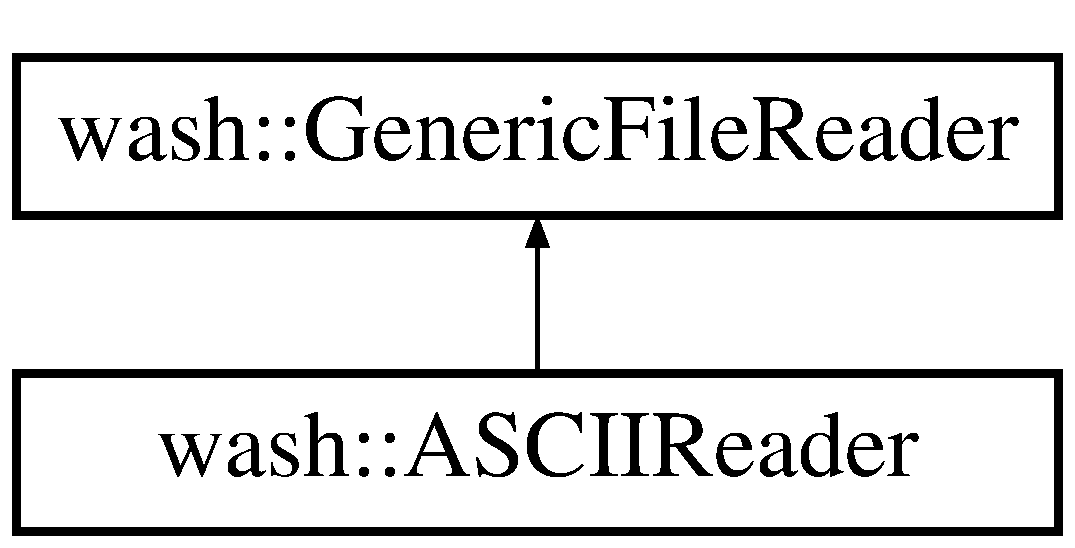
\includegraphics[height=2.000000cm]{classwash_1_1GenericFileReader}
\end{center}
\end{figure}
\subsection*{Public Member Functions}
\begin{DoxyCompactItemize}
\item 
\mbox{\Hypertarget{classwash_1_1GenericFileReader_a4be5668152706252a4d5759568cf4062}\label{classwash_1_1GenericFileReader_a4be5668152706252a4d5759568cf4062}} 
virtual void {\bfseries read\+\_\+iteration} (const size\+\_\+t iteration\+\_\+number) const =0
\end{DoxyCompactItemize}


The documentation for this class was generated from the following file\+:\begin{DoxyCompactItemize}
\item 
/dcs/20/u2002000/4th\+Year\+Project/wash/src/io/io.\+hpp\end{DoxyCompactItemize}

\hypertarget{classwash_1_1GenericFileWriter}{}\section{wash\+:\+:Generic\+File\+Writer Class Reference}
\label{classwash_1_1GenericFileWriter}\index{wash\+::\+Generic\+File\+Writer@{wash\+::\+Generic\+File\+Writer}}
Inheritance diagram for wash\+:\+:Generic\+File\+Writer\+:\begin{figure}[H]
\begin{center}
\leavevmode
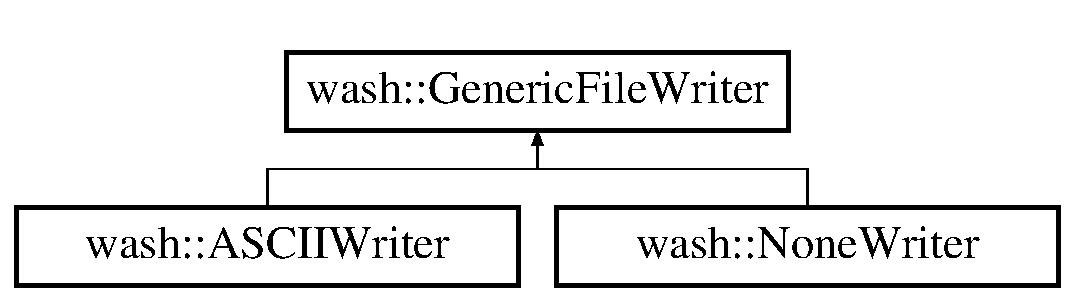
\includegraphics[height=2.000000cm]{classwash_1_1GenericFileWriter}
\end{center}
\end{figure}
\subsection*{Public Member Functions}
\begin{DoxyCompactItemize}
\item 
\mbox{\Hypertarget{classwash_1_1GenericFileWriter_aae09bd9ec13abb5c3935062e79338fef}\label{classwash_1_1GenericFileWriter_aae09bd9ec13abb5c3935062e79338fef}} 
virtual void {\bfseries write\+\_\+iteration} (const size\+\_\+t iterationc, const std\+::string path) const =0
\end{DoxyCompactItemize}


The documentation for this class was generated from the following file\+:\begin{DoxyCompactItemize}
\item 
/dcs/20/u2002000/4th\+Year\+Project/wash/src/io/io.\+hpp\end{DoxyCompactItemize}

\hypertarget{classwash_1_1Particle}{}\section{wash\+:\+:Particle Class Reference}
\label{classwash_1_1Particle}\index{wash\+::\+Particle@{wash\+::\+Particle}}


{\ttfamily \#include $<$particle.\+hpp$>$}

\subsection*{Public Member Functions}
\begin{DoxyCompactItemize}
\item 
\mbox{\hyperlink{classwash_1_1Particle_a72131cdf3fdbcada383d81604fd49503}{Particle}} (const unsigned local\+\_\+idx)
\begin{DoxyCompactList}\small\item\em T\+O\+DO\+: see if this works if it\textquotesingle{}s a glocal spec defined flag rather than in just one file? \end{DoxyCompactList}\item 
unsigned \mbox{\hyperlink{classwash_1_1Particle_aef9f2814cc392598de7756e1046fea67}{get\+\_\+id}} () const
\begin{DoxyCompactList}\small\item\em Returns the global ID of the particle. \end{DoxyCompactList}\item 
double \mbox{\hyperlink{classwash_1_1Particle_a8c0ce3f48b189fd8550c3bfab17eec68}{get\+\_\+density}} () const
\item 
void \mbox{\hyperlink{classwash_1_1Particle_a6416678dd509c16c2933d315b6ae6156}{set\+\_\+density}} (const double \mbox{\hyperlink{3d__fluid__sim_2fluid__sim_8cpp_a140d94d7edb97c062961056d1926a2db}{density}})
\item 
double \mbox{\hyperlink{classwash_1_1Particle_a7d8d11b3e4855e66e62ee58b4270cdc1}{get\+\_\+mass}} () const
\item 
void \mbox{\hyperlink{classwash_1_1Particle_a9151ed34c880f63f062381076834223e}{set\+\_\+mass}} (const double mass)
\item 
double \mbox{\hyperlink{classwash_1_1Particle_aab02f56502c6521382cf7a7320abc341}{get\+\_\+smoothing\+\_\+length}} () const
\item 
void \mbox{\hyperlink{classwash_1_1Particle_a15892a4346c05de955f91087dc88786d}{set\+\_\+smoothing\+\_\+length}} (const double smoothing\+\_\+length)
\item 
\mbox{\hyperlink{namespacewash_ab2cbbc37941b733095c9225b49b4cad9}{Simulation\+VecT}} \mbox{\hyperlink{classwash_1_1Particle_a9d222d453d640cf629ee8dfbee6b43c2}{get\+\_\+pos}} () const
\item 
void \mbox{\hyperlink{classwash_1_1Particle_af06835533935c04e594c258a7dcdd1ef}{set\+\_\+pos}} (const \mbox{\hyperlink{namespacewash_ab2cbbc37941b733095c9225b49b4cad9}{Simulation\+VecT}} pos)
\item 
\mbox{\hyperlink{namespacewash_ab2cbbc37941b733095c9225b49b4cad9}{Simulation\+VecT}} \mbox{\hyperlink{classwash_1_1Particle_a890d0f1467225393e385872b0c98b974}{get\+\_\+vel}} () const
\item 
void \mbox{\hyperlink{classwash_1_1Particle_a4755365883cfd62117ebe74fe44d35e0}{set\+\_\+vel}} (const \mbox{\hyperlink{namespacewash_ab2cbbc37941b733095c9225b49b4cad9}{Simulation\+VecT}} vel)
\item 
\mbox{\hyperlink{namespacewash_ab2cbbc37941b733095c9225b49b4cad9}{Simulation\+VecT}} \mbox{\hyperlink{classwash_1_1Particle_afb8c9dce2692cdfab61a3a87fde50610}{get\+\_\+acc}} () const
\item 
void \mbox{\hyperlink{classwash_1_1Particle_a395e095de0b2af7dfc925bedef2090a1}{set\+\_\+acc}} (const \mbox{\hyperlink{namespacewash_ab2cbbc37941b733095c9225b49b4cad9}{Simulation\+VecT}} acc)
\item 
double \mbox{\hyperlink{classwash_1_1Particle_ab42a162b41a4e8cf6212bd9c43f3a0cf}{get\+\_\+force\+\_\+scalar}} (const std\+::string \&force) const
\item 
void \mbox{\hyperlink{classwash_1_1Particle_a2c3038c8eac34e371922bcf1ab79b8ca}{set\+\_\+force\+\_\+scalar}} (const std\+::string \&force, const double value)
\item 
\mbox{\hyperlink{namespacewash_ab2cbbc37941b733095c9225b49b4cad9}{Simulation\+VecT}} \mbox{\hyperlink{classwash_1_1Particle_a9c6ec5d5a7407897ecca00549bd05c01}{get\+\_\+force\+\_\+vector}} (const std\+::string \&force) const
\item 
void \mbox{\hyperlink{classwash_1_1Particle_a6960cdd169d1829a52e49cf835a8bfeb}{set\+\_\+force\+\_\+vector}} (const std\+::string \&force, const \mbox{\hyperlink{namespacewash_ab2cbbc37941b733095c9225b49b4cad9}{Simulation\+VecT}} value)
\item 
double \mbox{\hyperlink{classwash_1_1Particle_ab16021a2c003de07dc0a418ffc3d5eb7}{get\+\_\+vol}} () const
\item 
unsigned \mbox{\hyperlink{classwash_1_1Particle_a570fc3286ab83d081950a5fb3d548d92}{recalculate\+\_\+neighbors}} (unsigned max\+\_\+count) const
\item 
bool \mbox{\hyperlink{classwash_1_1Particle_a32369e6edba4277ebc71917a37c2503d}{operator==}} (const \mbox{\hyperlink{classwash_1_1Particle}{Particle}} \&other) const
\begin{DoxyCompactList}\small\item\em Compare particle equality by their I\+Ds. \end{DoxyCompactList}\item 
bool \mbox{\hyperlink{classwash_1_1Particle_a32f1334a8a0b273a57355956d7e9fe63}{operator!=}} (const \mbox{\hyperlink{classwash_1_1Particle}{Particle}} \&other) const
\begin{DoxyCompactList}\small\item\em Inverse of equality check. \end{DoxyCompactList}\item 
\mbox{\hyperlink{classwash_1_1Particle_a9ca04366cb7412e6aa5d1d89108a8520}{Particle}} (const \mbox{\hyperlink{classwash_1_1Particle}{Particle}} \&)=delete
\item 
\mbox{\hyperlink{classwash_1_1Particle}{Particle}} \& \mbox{\hyperlink{classwash_1_1Particle_a8ac44cec043e444a45ab189f666f9d4b}{operator=}} (const \mbox{\hyperlink{classwash_1_1Particle}{Particle}} \&)=delete
\end{DoxyCompactItemize}
\subsection*{Friends}
\begin{DoxyCompactItemize}
\item 
std\+::ostream \& \mbox{\hyperlink{classwash_1_1Particle_ad7d60c63b6d14d1d0d4fe42d4e9dc8bc}{operator$<$$<$}} (std\+::ostream \&os, const \mbox{\hyperlink{classwash_1_1Particle}{Particle}} \&p)
\end{DoxyCompactItemize}


\subsection{Constructor \& Destructor Documentation}
\mbox{\Hypertarget{classwash_1_1Particle_a72131cdf3fdbcada383d81604fd49503}\label{classwash_1_1Particle_a72131cdf3fdbcada383d81604fd49503}} 
\index{wash\+::\+Particle@{wash\+::\+Particle}!Particle@{Particle}}
\index{Particle@{Particle}!wash\+::\+Particle@{wash\+::\+Particle}}
\subsubsection{\texorpdfstring{Particle()}{Particle()}\hspace{0.1cm}{\footnotesize\ttfamily [1/2]}}
{\footnotesize\ttfamily wash\+::\+Particle\+::\+Particle (\begin{DoxyParamCaption}\item[{const unsigned}]{local\+\_\+idx }\end{DoxyParamCaption})}



T\+O\+DO\+: see if this works if it\textquotesingle{}s a glocal spec defined flag rather than in just one file? 

\mbox{\Hypertarget{classwash_1_1Particle_a9ca04366cb7412e6aa5d1d89108a8520}\label{classwash_1_1Particle_a9ca04366cb7412e6aa5d1d89108a8520}} 
\index{wash\+::\+Particle@{wash\+::\+Particle}!Particle@{Particle}}
\index{Particle@{Particle}!wash\+::\+Particle@{wash\+::\+Particle}}
\subsubsection{\texorpdfstring{Particle()}{Particle()}\hspace{0.1cm}{\footnotesize\ttfamily [2/2]}}
{\footnotesize\ttfamily wash\+::\+Particle\+::\+Particle (\begin{DoxyParamCaption}\item[{const \mbox{\hyperlink{classwash_1_1Particle}{Particle}} \&}]{ }\end{DoxyParamCaption})\hspace{0.3cm}{\ttfamily [delete]}}



\subsection{Member Function Documentation}
\mbox{\Hypertarget{classwash_1_1Particle_afb8c9dce2692cdfab61a3a87fde50610}\label{classwash_1_1Particle_afb8c9dce2692cdfab61a3a87fde50610}} 
\index{wash\+::\+Particle@{wash\+::\+Particle}!get\+\_\+acc@{get\+\_\+acc}}
\index{get\+\_\+acc@{get\+\_\+acc}!wash\+::\+Particle@{wash\+::\+Particle}}
\subsubsection{\texorpdfstring{get\+\_\+acc()}{get\_acc()}}
{\footnotesize\ttfamily \mbox{\hyperlink{namespacewash_ab2cbbc37941b733095c9225b49b4cad9}{Simulation\+VecT}} wash\+::\+Particle\+::get\+\_\+acc (\begin{DoxyParamCaption}{ }\end{DoxyParamCaption}) const}

\mbox{\Hypertarget{classwash_1_1Particle_a8c0ce3f48b189fd8550c3bfab17eec68}\label{classwash_1_1Particle_a8c0ce3f48b189fd8550c3bfab17eec68}} 
\index{wash\+::\+Particle@{wash\+::\+Particle}!get\+\_\+density@{get\+\_\+density}}
\index{get\+\_\+density@{get\+\_\+density}!wash\+::\+Particle@{wash\+::\+Particle}}
\subsubsection{\texorpdfstring{get\+\_\+density()}{get\_density()}}
{\footnotesize\ttfamily double wash\+::\+Particle\+::get\+\_\+density (\begin{DoxyParamCaption}{ }\end{DoxyParamCaption}) const}

\mbox{\Hypertarget{classwash_1_1Particle_ab42a162b41a4e8cf6212bd9c43f3a0cf}\label{classwash_1_1Particle_ab42a162b41a4e8cf6212bd9c43f3a0cf}} 
\index{wash\+::\+Particle@{wash\+::\+Particle}!get\+\_\+force\+\_\+scalar@{get\+\_\+force\+\_\+scalar}}
\index{get\+\_\+force\+\_\+scalar@{get\+\_\+force\+\_\+scalar}!wash\+::\+Particle@{wash\+::\+Particle}}
\subsubsection{\texorpdfstring{get\+\_\+force\+\_\+scalar()}{get\_force\_scalar()}}
{\footnotesize\ttfamily double wash\+::\+Particle\+::get\+\_\+force\+\_\+scalar (\begin{DoxyParamCaption}\item[{const std\+::string \&}]{force }\end{DoxyParamCaption}) const}

\mbox{\Hypertarget{classwash_1_1Particle_a9c6ec5d5a7407897ecca00549bd05c01}\label{classwash_1_1Particle_a9c6ec5d5a7407897ecca00549bd05c01}} 
\index{wash\+::\+Particle@{wash\+::\+Particle}!get\+\_\+force\+\_\+vector@{get\+\_\+force\+\_\+vector}}
\index{get\+\_\+force\+\_\+vector@{get\+\_\+force\+\_\+vector}!wash\+::\+Particle@{wash\+::\+Particle}}
\subsubsection{\texorpdfstring{get\+\_\+force\+\_\+vector()}{get\_force\_vector()}}
{\footnotesize\ttfamily \mbox{\hyperlink{namespacewash_ab2cbbc37941b733095c9225b49b4cad9}{Simulation\+VecT}} wash\+::\+Particle\+::get\+\_\+force\+\_\+vector (\begin{DoxyParamCaption}\item[{const std\+::string \&}]{force }\end{DoxyParamCaption}) const}

\mbox{\Hypertarget{classwash_1_1Particle_aef9f2814cc392598de7756e1046fea67}\label{classwash_1_1Particle_aef9f2814cc392598de7756e1046fea67}} 
\index{wash\+::\+Particle@{wash\+::\+Particle}!get\+\_\+id@{get\+\_\+id}}
\index{get\+\_\+id@{get\+\_\+id}!wash\+::\+Particle@{wash\+::\+Particle}}
\subsubsection{\texorpdfstring{get\+\_\+id()}{get\_id()}}
{\footnotesize\ttfamily unsigned wash\+::\+Particle\+::get\+\_\+id (\begin{DoxyParamCaption}{ }\end{DoxyParamCaption}) const}



Returns the global ID of the particle. 

\mbox{\Hypertarget{classwash_1_1Particle_a7d8d11b3e4855e66e62ee58b4270cdc1}\label{classwash_1_1Particle_a7d8d11b3e4855e66e62ee58b4270cdc1}} 
\index{wash\+::\+Particle@{wash\+::\+Particle}!get\+\_\+mass@{get\+\_\+mass}}
\index{get\+\_\+mass@{get\+\_\+mass}!wash\+::\+Particle@{wash\+::\+Particle}}
\subsubsection{\texorpdfstring{get\+\_\+mass()}{get\_mass()}}
{\footnotesize\ttfamily double wash\+::\+Particle\+::get\+\_\+mass (\begin{DoxyParamCaption}{ }\end{DoxyParamCaption}) const}

\mbox{\Hypertarget{classwash_1_1Particle_a9d222d453d640cf629ee8dfbee6b43c2}\label{classwash_1_1Particle_a9d222d453d640cf629ee8dfbee6b43c2}} 
\index{wash\+::\+Particle@{wash\+::\+Particle}!get\+\_\+pos@{get\+\_\+pos}}
\index{get\+\_\+pos@{get\+\_\+pos}!wash\+::\+Particle@{wash\+::\+Particle}}
\subsubsection{\texorpdfstring{get\+\_\+pos()}{get\_pos()}}
{\footnotesize\ttfamily \mbox{\hyperlink{namespacewash_ab2cbbc37941b733095c9225b49b4cad9}{Simulation\+VecT}} wash\+::\+Particle\+::get\+\_\+pos (\begin{DoxyParamCaption}{ }\end{DoxyParamCaption}) const}

\mbox{\Hypertarget{classwash_1_1Particle_aab02f56502c6521382cf7a7320abc341}\label{classwash_1_1Particle_aab02f56502c6521382cf7a7320abc341}} 
\index{wash\+::\+Particle@{wash\+::\+Particle}!get\+\_\+smoothing\+\_\+length@{get\+\_\+smoothing\+\_\+length}}
\index{get\+\_\+smoothing\+\_\+length@{get\+\_\+smoothing\+\_\+length}!wash\+::\+Particle@{wash\+::\+Particle}}
\subsubsection{\texorpdfstring{get\+\_\+smoothing\+\_\+length()}{get\_smoothing\_length()}}
{\footnotesize\ttfamily double wash\+::\+Particle\+::get\+\_\+smoothing\+\_\+length (\begin{DoxyParamCaption}{ }\end{DoxyParamCaption}) const}

\mbox{\Hypertarget{classwash_1_1Particle_a890d0f1467225393e385872b0c98b974}\label{classwash_1_1Particle_a890d0f1467225393e385872b0c98b974}} 
\index{wash\+::\+Particle@{wash\+::\+Particle}!get\+\_\+vel@{get\+\_\+vel}}
\index{get\+\_\+vel@{get\+\_\+vel}!wash\+::\+Particle@{wash\+::\+Particle}}
\subsubsection{\texorpdfstring{get\+\_\+vel()}{get\_vel()}}
{\footnotesize\ttfamily \mbox{\hyperlink{namespacewash_ab2cbbc37941b733095c9225b49b4cad9}{Simulation\+VecT}} wash\+::\+Particle\+::get\+\_\+vel (\begin{DoxyParamCaption}{ }\end{DoxyParamCaption}) const}

\mbox{\Hypertarget{classwash_1_1Particle_ab16021a2c003de07dc0a418ffc3d5eb7}\label{classwash_1_1Particle_ab16021a2c003de07dc0a418ffc3d5eb7}} 
\index{wash\+::\+Particle@{wash\+::\+Particle}!get\+\_\+vol@{get\+\_\+vol}}
\index{get\+\_\+vol@{get\+\_\+vol}!wash\+::\+Particle@{wash\+::\+Particle}}
\subsubsection{\texorpdfstring{get\+\_\+vol()}{get\_vol()}}
{\footnotesize\ttfamily double wash\+::\+Particle\+::get\+\_\+vol (\begin{DoxyParamCaption}{ }\end{DoxyParamCaption}) const}

\mbox{\Hypertarget{classwash_1_1Particle_a32f1334a8a0b273a57355956d7e9fe63}\label{classwash_1_1Particle_a32f1334a8a0b273a57355956d7e9fe63}} 
\index{wash\+::\+Particle@{wash\+::\+Particle}!operator"!=@{operator"!=}}
\index{operator"!=@{operator"!=}!wash\+::\+Particle@{wash\+::\+Particle}}
\subsubsection{\texorpdfstring{operator"!=()}{operator!=()}}
{\footnotesize\ttfamily bool wash\+::\+Particle\+::operator!= (\begin{DoxyParamCaption}\item[{const \mbox{\hyperlink{classwash_1_1Particle}{Particle}} \&}]{other }\end{DoxyParamCaption}) const}



Inverse of equality check. 


\begin{DoxyParams}{Parameters}
{\em other} & \\
\hline
\end{DoxyParams}
\begin{DoxyReturn}{Returns}
true 

false 
\end{DoxyReturn}
\mbox{\Hypertarget{classwash_1_1Particle_a8ac44cec043e444a45ab189f666f9d4b}\label{classwash_1_1Particle_a8ac44cec043e444a45ab189f666f9d4b}} 
\index{wash\+::\+Particle@{wash\+::\+Particle}!operator=@{operator=}}
\index{operator=@{operator=}!wash\+::\+Particle@{wash\+::\+Particle}}
\subsubsection{\texorpdfstring{operator=()}{operator=()}}
{\footnotesize\ttfamily \mbox{\hyperlink{classwash_1_1Particle}{Particle}}\& wash\+::\+Particle\+::operator= (\begin{DoxyParamCaption}\item[{const \mbox{\hyperlink{classwash_1_1Particle}{Particle}} \&}]{ }\end{DoxyParamCaption})\hspace{0.3cm}{\ttfamily [delete]}}

\mbox{\Hypertarget{classwash_1_1Particle_a32369e6edba4277ebc71917a37c2503d}\label{classwash_1_1Particle_a32369e6edba4277ebc71917a37c2503d}} 
\index{wash\+::\+Particle@{wash\+::\+Particle}!operator==@{operator==}}
\index{operator==@{operator==}!wash\+::\+Particle@{wash\+::\+Particle}}
\subsubsection{\texorpdfstring{operator==()}{operator==()}}
{\footnotesize\ttfamily bool wash\+::\+Particle\+::operator== (\begin{DoxyParamCaption}\item[{const \mbox{\hyperlink{classwash_1_1Particle}{Particle}} \&}]{other }\end{DoxyParamCaption}) const}



Compare particle equality by their I\+Ds. 


\begin{DoxyParams}{Parameters}
{\em other} & \\
\hline
\end{DoxyParams}
\begin{DoxyReturn}{Returns}
true ID\textquotesingle{}s equal 

false ID\textquotesingle{}s not equal 
\end{DoxyReturn}
\mbox{\Hypertarget{classwash_1_1Particle_a570fc3286ab83d081950a5fb3d548d92}\label{classwash_1_1Particle_a570fc3286ab83d081950a5fb3d548d92}} 
\index{wash\+::\+Particle@{wash\+::\+Particle}!recalculate\+\_\+neighbors@{recalculate\+\_\+neighbors}}
\index{recalculate\+\_\+neighbors@{recalculate\+\_\+neighbors}!wash\+::\+Particle@{wash\+::\+Particle}}
\subsubsection{\texorpdfstring{recalculate\+\_\+neighbors()}{recalculate\_neighbors()}}
{\footnotesize\ttfamily unsigned wash\+::\+Particle\+::recalculate\+\_\+neighbors (\begin{DoxyParamCaption}\item[{unsigned}]{max\+\_\+count }\end{DoxyParamCaption}) const}

\mbox{\Hypertarget{classwash_1_1Particle_a395e095de0b2af7dfc925bedef2090a1}\label{classwash_1_1Particle_a395e095de0b2af7dfc925bedef2090a1}} 
\index{wash\+::\+Particle@{wash\+::\+Particle}!set\+\_\+acc@{set\+\_\+acc}}
\index{set\+\_\+acc@{set\+\_\+acc}!wash\+::\+Particle@{wash\+::\+Particle}}
\subsubsection{\texorpdfstring{set\+\_\+acc()}{set\_acc()}}
{\footnotesize\ttfamily void wash\+::\+Particle\+::set\+\_\+acc (\begin{DoxyParamCaption}\item[{const \mbox{\hyperlink{namespacewash_ab2cbbc37941b733095c9225b49b4cad9}{Simulation\+VecT}}}]{acc }\end{DoxyParamCaption})}

\mbox{\Hypertarget{classwash_1_1Particle_a6416678dd509c16c2933d315b6ae6156}\label{classwash_1_1Particle_a6416678dd509c16c2933d315b6ae6156}} 
\index{wash\+::\+Particle@{wash\+::\+Particle}!set\+\_\+density@{set\+\_\+density}}
\index{set\+\_\+density@{set\+\_\+density}!wash\+::\+Particle@{wash\+::\+Particle}}
\subsubsection{\texorpdfstring{set\+\_\+density()}{set\_density()}}
{\footnotesize\ttfamily void wash\+::\+Particle\+::set\+\_\+density (\begin{DoxyParamCaption}\item[{const double}]{density }\end{DoxyParamCaption})}

\mbox{\Hypertarget{classwash_1_1Particle_a2c3038c8eac34e371922bcf1ab79b8ca}\label{classwash_1_1Particle_a2c3038c8eac34e371922bcf1ab79b8ca}} 
\index{wash\+::\+Particle@{wash\+::\+Particle}!set\+\_\+force\+\_\+scalar@{set\+\_\+force\+\_\+scalar}}
\index{set\+\_\+force\+\_\+scalar@{set\+\_\+force\+\_\+scalar}!wash\+::\+Particle@{wash\+::\+Particle}}
\subsubsection{\texorpdfstring{set\+\_\+force\+\_\+scalar()}{set\_force\_scalar()}}
{\footnotesize\ttfamily void wash\+::\+Particle\+::set\+\_\+force\+\_\+scalar (\begin{DoxyParamCaption}\item[{const std\+::string \&}]{force,  }\item[{const double}]{value }\end{DoxyParamCaption})}

\mbox{\Hypertarget{classwash_1_1Particle_a6960cdd169d1829a52e49cf835a8bfeb}\label{classwash_1_1Particle_a6960cdd169d1829a52e49cf835a8bfeb}} 
\index{wash\+::\+Particle@{wash\+::\+Particle}!set\+\_\+force\+\_\+vector@{set\+\_\+force\+\_\+vector}}
\index{set\+\_\+force\+\_\+vector@{set\+\_\+force\+\_\+vector}!wash\+::\+Particle@{wash\+::\+Particle}}
\subsubsection{\texorpdfstring{set\+\_\+force\+\_\+vector()}{set\_force\_vector()}}
{\footnotesize\ttfamily void wash\+::\+Particle\+::set\+\_\+force\+\_\+vector (\begin{DoxyParamCaption}\item[{const std\+::string \&}]{force,  }\item[{const \mbox{\hyperlink{namespacewash_ab2cbbc37941b733095c9225b49b4cad9}{Simulation\+VecT}}}]{value }\end{DoxyParamCaption})}

\mbox{\Hypertarget{classwash_1_1Particle_a9151ed34c880f63f062381076834223e}\label{classwash_1_1Particle_a9151ed34c880f63f062381076834223e}} 
\index{wash\+::\+Particle@{wash\+::\+Particle}!set\+\_\+mass@{set\+\_\+mass}}
\index{set\+\_\+mass@{set\+\_\+mass}!wash\+::\+Particle@{wash\+::\+Particle}}
\subsubsection{\texorpdfstring{set\+\_\+mass()}{set\_mass()}}
{\footnotesize\ttfamily void wash\+::\+Particle\+::set\+\_\+mass (\begin{DoxyParamCaption}\item[{const double}]{mass }\end{DoxyParamCaption})}

\mbox{\Hypertarget{classwash_1_1Particle_af06835533935c04e594c258a7dcdd1ef}\label{classwash_1_1Particle_af06835533935c04e594c258a7dcdd1ef}} 
\index{wash\+::\+Particle@{wash\+::\+Particle}!set\+\_\+pos@{set\+\_\+pos}}
\index{set\+\_\+pos@{set\+\_\+pos}!wash\+::\+Particle@{wash\+::\+Particle}}
\subsubsection{\texorpdfstring{set\+\_\+pos()}{set\_pos()}}
{\footnotesize\ttfamily void wash\+::\+Particle\+::set\+\_\+pos (\begin{DoxyParamCaption}\item[{const \mbox{\hyperlink{namespacewash_ab2cbbc37941b733095c9225b49b4cad9}{Simulation\+VecT}}}]{pos }\end{DoxyParamCaption})}

\mbox{\Hypertarget{classwash_1_1Particle_a15892a4346c05de955f91087dc88786d}\label{classwash_1_1Particle_a15892a4346c05de955f91087dc88786d}} 
\index{wash\+::\+Particle@{wash\+::\+Particle}!set\+\_\+smoothing\+\_\+length@{set\+\_\+smoothing\+\_\+length}}
\index{set\+\_\+smoothing\+\_\+length@{set\+\_\+smoothing\+\_\+length}!wash\+::\+Particle@{wash\+::\+Particle}}
\subsubsection{\texorpdfstring{set\+\_\+smoothing\+\_\+length()}{set\_smoothing\_length()}}
{\footnotesize\ttfamily void wash\+::\+Particle\+::set\+\_\+smoothing\+\_\+length (\begin{DoxyParamCaption}\item[{const double}]{smoothing\+\_\+length }\end{DoxyParamCaption})}

\mbox{\Hypertarget{classwash_1_1Particle_a4755365883cfd62117ebe74fe44d35e0}\label{classwash_1_1Particle_a4755365883cfd62117ebe74fe44d35e0}} 
\index{wash\+::\+Particle@{wash\+::\+Particle}!set\+\_\+vel@{set\+\_\+vel}}
\index{set\+\_\+vel@{set\+\_\+vel}!wash\+::\+Particle@{wash\+::\+Particle}}
\subsubsection{\texorpdfstring{set\+\_\+vel()}{set\_vel()}}
{\footnotesize\ttfamily void wash\+::\+Particle\+::set\+\_\+vel (\begin{DoxyParamCaption}\item[{const \mbox{\hyperlink{namespacewash_ab2cbbc37941b733095c9225b49b4cad9}{Simulation\+VecT}}}]{vel }\end{DoxyParamCaption})}



\subsection{Friends And Related Function Documentation}
\mbox{\Hypertarget{classwash_1_1Particle_ad7d60c63b6d14d1d0d4fe42d4e9dc8bc}\label{classwash_1_1Particle_ad7d60c63b6d14d1d0d4fe42d4e9dc8bc}} 
\index{wash\+::\+Particle@{wash\+::\+Particle}!operator$<$$<$@{operator$<$$<$}}
\index{operator$<$$<$@{operator$<$$<$}!wash\+::\+Particle@{wash\+::\+Particle}}
\subsubsection{\texorpdfstring{operator$<$$<$}{operator<<}}
{\footnotesize\ttfamily std\+::ostream\& operator$<$$<$ (\begin{DoxyParamCaption}\item[{std\+::ostream \&}]{os,  }\item[{const \mbox{\hyperlink{classwash_1_1Particle}{Particle}} \&}]{p }\end{DoxyParamCaption})\hspace{0.3cm}{\ttfamily [friend]}}



The documentation for this class was generated from the following files\+:\begin{DoxyCompactItemize}
\item 
/dcs/20/u2002000/4th\+Year\+Project/wash/include/\mbox{\hyperlink{particle_8hpp}{particle.\+hpp}}\item 
/dcs/20/u2002000/4th\+Year\+Project/wash/src/impl/cstone/\mbox{\hyperlink{cstone_2particle_8cpp}{particle.\+cpp}}\end{DoxyCompactItemize}

\hypertarget{classwash_1_1Vec}{}\section{wash\+:\+:Vec$<$ T, dim $>$ Class Template Reference}
\label{classwash_1_1Vec}\index{wash\+::\+Vec$<$ T, dim $>$@{wash\+::\+Vec$<$ T, dim $>$}}
\subsection*{Public Member Functions}
\begin{DoxyCompactItemize}
\item 
\mbox{\Hypertarget{classwash_1_1Vec_a6250ba5f027e9e0e974654136ea7e6ef}\label{classwash_1_1Vec_a6250ba5f027e9e0e974654136ea7e6ef}} 
{\bfseries Vec} (std\+::initializer\+\_\+list$<$ T $>$ l)
\item 
\mbox{\Hypertarget{classwash_1_1Vec_a5927d6caa8489a88b8470fe8bb8779d0}\label{classwash_1_1Vec_a5927d6caa8489a88b8470fe8bb8779d0}} 
T $\ast$ {\bfseries operator\mbox{[}$\,$\mbox{]}} (int i)
\item 
\mbox{\Hypertarget{classwash_1_1Vec_ad8a8863138b26c2b2eae41e11f40e78f}\label{classwash_1_1Vec_ad8a8863138b26c2b2eae41e11f40e78f}} 
\mbox{\hyperlink{classwash_1_1Vec}{Vec}}$<$ T, dim $>$ {\bfseries operator+} (T d)
\item 
\mbox{\Hypertarget{classwash_1_1Vec_a951a842c43b3cf99d60abfe73e53475c}\label{classwash_1_1Vec_a951a842c43b3cf99d60abfe73e53475c}} 
\mbox{\hyperlink{classwash_1_1Vec}{Vec}}$<$ T, dim $>$ {\bfseries operator+} (\mbox{\hyperlink{classwash_1_1Vec}{Vec}}$<$ T, dim $>$ v)
\item 
\mbox{\Hypertarget{classwash_1_1Vec_ac92d90da0a36cdd6b38a8a12e341fa84}\label{classwash_1_1Vec_ac92d90da0a36cdd6b38a8a12e341fa84}} 
void {\bfseries operator+=} (\mbox{\hyperlink{classwash_1_1Vec}{Vec}}$<$ T, dim $>$ v)
\item 
\mbox{\Hypertarget{classwash_1_1Vec_a83a86542f9afb7ea0b5b7b8ab72eb119}\label{classwash_1_1Vec_a83a86542f9afb7ea0b5b7b8ab72eb119}} 
\mbox{\hyperlink{classwash_1_1Vec}{Vec}}$<$ T, dim $>$ {\bfseries operator-\/} (\mbox{\hyperlink{classwash_1_1Vec}{Vec}}$<$ T, dim $>$ v) const
\item 
\mbox{\Hypertarget{classwash_1_1Vec_a972cde51776de1a9efec7ed6ea02f401}\label{classwash_1_1Vec_a972cde51776de1a9efec7ed6ea02f401}} 
\mbox{\hyperlink{classwash_1_1Vec}{Vec}}$<$ T, dim $>$ {\bfseries operator/} (T d)
\item 
\mbox{\Hypertarget{classwash_1_1Vec_a6fc9e30b352c72c7307bd28ee6c0aa72}\label{classwash_1_1Vec_a6fc9e30b352c72c7307bd28ee6c0aa72}} 
\mbox{\hyperlink{classwash_1_1Vec}{Vec}}$<$ T, dim $>$ {\bfseries operator$\ast$} (T d)
\item 
\mbox{\Hypertarget{classwash_1_1Vec_a41de499daf12160b2cf515ce0c9da70f}\label{classwash_1_1Vec_a41de499daf12160b2cf515ce0c9da70f}} 
T {\bfseries magnitude} ()
\item 
\mbox{\Hypertarget{classwash_1_1Vec_a1be26013b6d4f898b8504fc258043400}\label{classwash_1_1Vec_a1be26013b6d4f898b8504fc258043400}} 
T {\bfseries at} (const size\+\_\+t i) const
\item 
\mbox{\Hypertarget{classwash_1_1Vec_aae15a1a2cea7e883e53c2e7f6164710a}\label{classwash_1_1Vec_aae15a1a2cea7e883e53c2e7f6164710a}} 
\mbox{\hyperlink{classwash_1_1Vec}{Vec}}$<$ T, dim $>$ {\bfseries abs} () const
\end{DoxyCompactItemize}


The documentation for this class was generated from the following file\+:\begin{DoxyCompactItemize}
\item 
/dcs/20/u2002000/4th\+Year\+Project/wash/wash\+\_\+vector.\+hpp\end{DoxyCompactItemize}

\chapter{File Documentation}
\hypertarget{mock__io_8hpp}{}\section{/dcs/20/u2002000/4th\+Year\+Project/wash/io/mock\+\_\+io.hpp File Reference}
\label{mock__io_8hpp}\index{/dcs/20/u2002000/4th\+Year\+Project/wash/io/mock\+\_\+io.\+hpp@{/dcs/20/u2002000/4th\+Year\+Project/wash/io/mock\+\_\+io.\+hpp}}


Provides declarations for A\+PI functions dealing with file IO in the serial mock-\/up.  


{\ttfamily \#include $<$iostream$>$}\newline
{\ttfamily \#include \char`\"{}../wash\+\_\+mockapi.\+hpp\char`\"{}}\newline
\subsection*{Classes}
\begin{DoxyCompactItemize}
\item 
class \mbox{\hyperlink{classwash_1_1GenericFileWriter}{wash\+::\+Generic\+File\+Writer}}
\item 
class \mbox{\hyperlink{classwash_1_1GenericFileReader}{wash\+::\+Generic\+File\+Reader}}
\end{DoxyCompactItemize}
\subsection*{Functions}
\begin{DoxyCompactItemize}
\item 
std\+::unique\+\_\+ptr$<$ Generic\+File\+Writer $>$ {\bfseries wash\+::get\+\_\+file\+\_\+writer} (const std\+::string format)
\begin{DoxyCompactList}\small\item\em Get the file writer object for a given format. \end{DoxyCompactList}\item 
std\+::unique\+\_\+ptr$<$ Generic\+File\+Reader $>$ {\bfseries wash\+::get\+\_\+file\+\_\+reader} (const std\+::string format)
\begin{DoxyCompactList}\small\item\em Get the file reader object based on the format. \end{DoxyCompactList}\end{DoxyCompactItemize}


\subsection{Detailed Description}
Provides declarations for A\+PI functions dealing with file IO in the serial mock-\/up. 

\begin{DoxyAuthor}{Author}
James Macer-\/\+Wright 
\end{DoxyAuthor}
\begin{DoxyVersion}{Version}
0.\+1 
\end{DoxyVersion}
\begin{DoxyDate}{Date}
2023-\/11-\/15
\end{DoxyDate}
\begin{DoxyCopyright}{Copyright}
Copyright (c) 2023
\end{DoxyCopyright}
Provides several functions useful for outputting the data to a file periodically, and reading data from those files to continue the simulation from a \char`\"{}checkpoint\char`\"{}

Currently, supports in the implementation H\+D\+F5 or ascii (plaintext) file outputs. 

\subsection{Function Documentation}
\mbox{\Hypertarget{mock__io_8cpp_file_ad641b75009f166b30560b3fa61f0f9eb}\label{mock__io_8cpp_file_ad641b75009f166b30560b3fa61f0f9eb}} 
\index{mock\+\_\+io.\+hpp@{mock\+\_\+io.\+hpp}!get\+\_\+file\+\_\+reader@{get\+\_\+file\+\_\+reader}}
\index{get\+\_\+file\+\_\+reader@{get\+\_\+file\+\_\+reader}!mock\+\_\+io.\+hpp@{mock\+\_\+io.\+hpp}}
\subsubsection{\texorpdfstring{get\+\_\+file\+\_\+reader()}{get\_file\_reader()}}
{\footnotesize\ttfamily std\+::unique\+\_\+ptr$<$ Generic\+File\+Reader $>$ wash\+::get\+\_\+file\+\_\+reader (\begin{DoxyParamCaption}\item[{const std\+::string}]{format }\end{DoxyParamCaption})}



Get the file reader object based on the format. 


\begin{DoxyParams}{Parameters}
{\em file\+\_\+name} & File format we want to read in \\
\hline
\end{DoxyParams}
\begin{DoxyReturn}{Returns}
Generic\+File\+Reader 
\end{DoxyReturn}
\mbox{\Hypertarget{mock__io_8cpp_file_a8d00d5b1a05d54f99a4105d5bf12e3ab}\label{mock__io_8cpp_file_a8d00d5b1a05d54f99a4105d5bf12e3ab}} 
\index{mock\+\_\+io.\+hpp@{mock\+\_\+io.\+hpp}!get\+\_\+file\+\_\+writer@{get\+\_\+file\+\_\+writer}}
\index{get\+\_\+file\+\_\+writer@{get\+\_\+file\+\_\+writer}!mock\+\_\+io.\+hpp@{mock\+\_\+io.\+hpp}}
\subsubsection{\texorpdfstring{get\+\_\+file\+\_\+writer()}{get\_file\_writer()}}
{\footnotesize\ttfamily std\+::unique\+\_\+ptr$<$ Generic\+File\+Writer $>$ wash\+::get\+\_\+file\+\_\+writer (\begin{DoxyParamCaption}\item[{const std\+::string}]{format }\end{DoxyParamCaption})}



Get the file writer object for a given format. 


\begin{DoxyParams}{Parameters}
{\em format} & File format we want to output as \\
\hline
\end{DoxyParams}
\begin{DoxyReturn}{Returns}
Generic\+File\+Writer 
\end{DoxyReturn}

\hypertarget{read__ascii_8cpp}{}\section{/dcs/20/u2002000/4th\+Year\+Project/wash/src/io/read\+\_\+ascii.cpp File Reference}
\label{read__ascii_8cpp}\index{/dcs/20/u2002000/4th\+Year\+Project/wash/src/io/read\+\_\+ascii.\+cpp@{/dcs/20/u2002000/4th\+Year\+Project/wash/src/io/read\+\_\+ascii.\+cpp}}


Reads in an ascii plaintext file into the simulation as a checkpoint.  


{\ttfamily \#include \char`\"{}ascii.\+hpp\char`\"{}}\newline


\subsection{Detailed Description}
Reads in an ascii plaintext file into the simulation as a checkpoint. 

\begin{DoxyAuthor}{Author}
James Macer-\/\+Wright 
\end{DoxyAuthor}
\begin{DoxyVersion}{Version}
0.\+1 
\end{DoxyVersion}
\begin{DoxyDate}{Date}
2023-\/11-\/15
\end{DoxyDate}
\begin{DoxyCopyright}{Copyright}
Copyright (c) 2023 
\end{DoxyCopyright}

\hypertarget{read__hdf5_8cpp}{}\section{/dcs/20/u2002000/4th\+Year\+Project/wash/src/io/read\+\_\+hdf5.cpp File Reference}
\label{read__hdf5_8cpp}\index{/dcs/20/u2002000/4th\+Year\+Project/wash/src/io/read\+\_\+hdf5.\+cpp@{/dcs/20/u2002000/4th\+Year\+Project/wash/src/io/read\+\_\+hdf5.\+cpp}}


Reads in a H\+D\+F5 file with the intention of constructing a simulation state from which to continue.  


{\ttfamily \#include \char`\"{}hdf5.\+hpp\char`\"{}}\newline


\subsection{Detailed Description}
Reads in a H\+D\+F5 file with the intention of constructing a simulation state from which to continue. 

\begin{DoxyAuthor}{Author}
James Macer-\/\+Wright 
\end{DoxyAuthor}
\begin{DoxyVersion}{Version}
0.\+1 
\end{DoxyVersion}
\begin{DoxyDate}{Date}
2023-\/11-\/15
\end{DoxyDate}
\begin{DoxyCopyright}{Copyright}
Copyright (c) 2023
\end{DoxyCopyright}
Occasionally, we might want to stop the computation of a simulation for various reasons eventually we will then want to restart the simulation starting from where we left of. 
\hypertarget{test__io_8cpp}{}\section{/dcs/20/u2002000/4th\+Year\+Project/wash/io/test\+\_\+io.cpp File Reference}
\label{test__io_8cpp}\index{/dcs/20/u2002000/4th\+Year\+Project/wash/io/test\+\_\+io.\+cpp@{/dcs/20/u2002000/4th\+Year\+Project/wash/io/test\+\_\+io.\+cpp}}


Tests the File IO methods currently implemented by writing dummy data out.  


{\ttfamily \#include \char`\"{}mock\+\_\+io.\+hpp\char`\"{}}\newline
\subsection*{Functions}
\begin{DoxyCompactItemize}
\item 
\mbox{\Hypertarget{test__io_8cpp_af5505694b33b44f3284f5cba8c1931cd}\label{test__io_8cpp_af5505694b33b44f3284f5cba8c1931cd}} 
void \mbox{\hyperlink{test__io_8cpp_af5505694b33b44f3284f5cba8c1931cd}{create\+\_\+particles}} (const size\+\_\+t num\+\_\+particles)
\begin{DoxyCompactList}\small\item\em Create a bunch of particles randomly for testing. \end{DoxyCompactList}\item 
\mbox{\Hypertarget{test__io_8cpp_a712a367fbd45b250c52dce663be28c1f}\label{test__io_8cpp_a712a367fbd45b250c52dce663be28c1f}} 
void \mbox{\hyperlink{test__io_8cpp_a712a367fbd45b250c52dce663be28c1f}{hdf5\+\_\+test}} ()
\begin{DoxyCompactList}\small\item\em Write out the dummy simulation state to a H\+D\+F5 file. \end{DoxyCompactList}\item 
\mbox{\Hypertarget{test__io_8cpp_a5af0ae84045ce72bd19f55d630168c42}\label{test__io_8cpp_a5af0ae84045ce72bd19f55d630168c42}} 
void \mbox{\hyperlink{test__io_8cpp_a5af0ae84045ce72bd19f55d630168c42}{ascii\+\_\+test}} ()
\begin{DoxyCompactList}\small\item\em Write out the dummy simulation state to an A\+S\+C\+II C\+SV file. \end{DoxyCompactList}\item 
\mbox{\Hypertarget{test__io_8cpp_a3c04138a5bfe5d72780bb7e82a18e627}\label{test__io_8cpp_a3c04138a5bfe5d72780bb7e82a18e627}} 
int {\bfseries main} (int argc, char $\ast$$\ast$argv)
\end{DoxyCompactItemize}


\subsection{Detailed Description}
Tests the File IO methods currently implemented by writing dummy data out. 

\begin{DoxyAuthor}{Author}
James Macer-\/\+Wright 
\end{DoxyAuthor}
\begin{DoxyVersion}{Version}
0.\+1 
\end{DoxyVersion}
\begin{DoxyDate}{Date}
2023-\/11-\/18
\end{DoxyDate}
\begin{DoxyCopyright}{Copyright}
Copyright (c) 2023 
\end{DoxyCopyright}

\hypertarget{write__ascii_8cpp}{}\section{/dcs/20/u2002000/4th\+Year\+Project/wash/src/io/write\+\_\+ascii.cpp File Reference}
\label{write__ascii_8cpp}\index{/dcs/20/u2002000/4th\+Year\+Project/wash/src/io/write\+\_\+ascii.\+cpp@{/dcs/20/u2002000/4th\+Year\+Project/wash/src/io/write\+\_\+ascii.\+cpp}}


Writes the simulation data to an ascii plaintext file in C\+SV format.  


{\ttfamily \#include $<$fstream$>$}\newline
{\ttfamily \#include \char`\"{}ascii.\+hpp\char`\"{}}\newline
\subsection*{Namespaces}
\begin{DoxyCompactItemize}
\item 
 \mbox{\hyperlink{namespacewash}{wash}}
\begin{DoxyCompactList}\small\item\em T\+O\+DO\+: Consider having this as a private header in W\+I\+S\+B/\+W\+S2\+S\+T/etc implementations. \end{DoxyCompactList}\item 
 \mbox{\hyperlink{namespacewash_1_1io}{wash\+::io}}
\end{DoxyCompactItemize}
\subsection*{Functions}
\begin{DoxyCompactItemize}
\item 
int \mbox{\hyperlink{namespacewash_1_1io_ab29d891bfd64999f5ffb3aa5b13c5b22}{wash\+::io\+::write\+\_\+ascii}} (const I\+O\+Manager \&io, const Simulation\+Data \&sim\+\_\+data, size\+\_\+t iter)
\begin{DoxyCompactList}\small\item\em Write A\+S\+C\+II Output. \end{DoxyCompactList}\end{DoxyCompactItemize}


\subsection{Detailed Description}
Writes the simulation data to an ascii plaintext file in C\+SV format. 

\begin{DoxyAuthor}{Author}
James Macer-\/\+Wright 
\end{DoxyAuthor}
\begin{DoxyVersion}{Version}
0.\+1 
\end{DoxyVersion}
\begin{DoxyDate}{Date}
2023-\/11-\/15
\end{DoxyDate}
\begin{DoxyCopyright}{Copyright}
Copyright (c) 2023 
\end{DoxyCopyright}

\hypertarget{write__hdf5_8cpp}{}\section{/dcs/20/u2002000/4th\+Year\+Project/wash/src/io/write\+\_\+hdf5.cpp File Reference}
\label{write__hdf5_8cpp}\index{/dcs/20/u2002000/4th\+Year\+Project/wash/src/io/write\+\_\+hdf5.\+cpp@{/dcs/20/u2002000/4th\+Year\+Project/wash/src/io/write\+\_\+hdf5.\+cpp}}


Write out the simulation state serially to a H\+D\+F5 file.  


{\ttfamily \#include \char`\"{}hdf5.\+hpp\char`\"{}}\newline


\subsection{Detailed Description}
Write out the simulation state serially to a H\+D\+F5 file. 

\begin{DoxyAuthor}{Author}
James Macer-\/\+Wright 
\end{DoxyAuthor}
\begin{DoxyVersion}{Version}
0.\+1 
\end{DoxyVersion}
\begin{DoxyDate}{Date}
2023-\/11-\/15
\end{DoxyDate}
\begin{DoxyCopyright}{Copyright}
Copyright (c) 2023
\end{DoxyCopyright}
Periodically we want to write out the simulation data to a file to inspect the intermediate values of particles \& properties. This can be achieved with a number of different backend technologies, H\+D\+F5 is one which supports parallelism with M\+PI.

As well, H\+D\+F5 formats can be read by visualisation software such as S\+P\+La\+SH which was built for visualising S\+PH simulation data.

We expect H\+D\+F5 to be built and present on the system for this use. 
%--- End generated contents ---

% Index
\backmatter
\newpage
\phantomsection
\clearemptydoublepage
\addcontentsline{toc}{chapter}{Index}
\printindex

\end{document}
